\documentclass{article}

\usepackage{fancyhdr} % Required for custom headers
\usepackage{lastpage} % Required to determine the last page for the footer
\usepackage{extramarks} % Required for headers and footers
\usepackage[usenames,dvipsnames]{color} % Required for custom colors
\usepackage{graphicx} % Required to insert images
\usepackage{listings} % Required for insertion of code
\usepackage{courier} % Required for the courier font
\usepackage{lipsum} % Used for inserting dummy 'Lorem ipsum' text into the template
\usepackage{hyperref}
\usepackage{xcolor}




\hypersetup{
    colorlinks=true,
    %linkbordercolor={white},
    %urlbordercolor={white},
    %runbordercolor={white},
    %citebordercolor={white},
    linkcolor={black},
    menucolor = {black},
    urlcolor = {blue},
    runcolor = {black},
    citecolor = {black},
    anchorcolor = {blue}
}

\topmargin=-0.45in
\evensidemargin=0in
\oddsidemargin=0in
\textwidth=6.5in
\textheight=9.0in
\headsep=0.25in

\linespread{1.1} % Line spacing

% Set up the header and footer
\pagestyle{fancy}
\lhead{\AssName} % Top left header
\rhead{\DocName} % Top right header
\lfoot{\DocRef} % Bottom left footer
\cfoot{email: team@apertus.org} % Bottom center footer
\rfoot{Page\ \thepage\ of\ \protect\pageref{LastPage}} % Bottom right footer
\renewcommand\headrulewidth{0.4pt} % Size of the header rule
\renewcommand\footrulewidth{0.4pt} % Size of the footer rule

\setlength\parindent{0pt} % Removes all indentation from paragraphs






%----------------------------------------------------------------------------------------
%	CODE CONFIGURATION
%----------------------------------------------------------------------------------------

\definecolor{MyDarkGreen}{rgb}{0.0,0.4,0.0} % This is the color used for comments
\lstloadlanguages{Perl} % Load Perl syntax for listings, for a list of other languages supported see: ftp://ftp.tex.ac.uk/tex-archive/macros/latex/contrib/listings/listings.pdf
\lstset{language=Perl, % Use Perl in this example
        frame=single, % Single frame around code
        basicstyle=\small\ttfamily, % Use small true type font
        keywordstyle=[1]\color{Blue}\bf, % Perl functions bold and blue
        keywordstyle=[2]\color{Purple}, % Perl function arguments purple
        keywordstyle=[3]\color{Blue}\underbar, % Custom functions underlined and blue
        identifierstyle=, % Nothing special about identifiers                                         
        commentstyle=\usefont{T1}{pcr}{m}{sl}\color{MyDarkGreen}\small, % Comments small dark green courier font
        stringstyle=\color{Purple}, % Strings are purple
        showstringspaces=false, % Don't put marks in string spaces
        tabsize=5, % 5 spaces per tab
        %
        % Put standard Perl functions not included in the default language here
        morekeywords={rand},
        %
        % Put Perl function parameters here
        morekeywords=[2]{on, off, interp},
        %
        % Put user defined functions here
        morekeywords=[3]{test},
       	%
        morecomment=[l][\color{Blue}]{...}, % Line continuation (...) like blue comment
        numbers=left, % Line numbers on left
        firstnumber=1, % Line numbers start with line 1
        numberstyle=\tiny\color{Blue}, % Line numbers are blue and small
        stepnumber=5 % Line numbers go in steps of 5
}

% Creates a new command to include a perl script, the first parameter is the filename of the script (without .pl), the second parameter is the caption
\newcommand{\perlscript}[2]{
\begin{itemize}
\item[]\lstinputlisting[caption=#2,label=#1]{#1.pl}
\end{itemize}
}

%----------------------------------------------------------------------------------------
%	STRUCTURE COMMANDS
%----------------------------------------------------------------------------------------

% Header and footer for when a page split occurs within a problem environment
\newcommand{\enterProblemHeader}[1]{
\nobreak\extramarks{#1}{#1 continued on next page\ldots}\nobreak
\nobreak\extramarks{#1 (continued)}{#1 continued on next page\ldots}\nobreak
}

% Header and footer for when a page split occurs between problem environments
\newcommand{\exitProblemHeader}[1]{
\nobreak\extramarks{#1 (continued)}{#1 continued on next page\ldots}\nobreak
\nobreak\extramarks{#1}{}\nobreak
}

\setcounter{secnumdepth}{5} % Makes sure that the indexing tree has 5 tiers
\setcounter{tocdepth}{5}

\newcommand{\homeworkProblemName}{}
\newenvironment{homeworkProblem}[1][Problem \arabic{homeworkProblemCounter}]{ % Makes a new environment called homeworkProblem which takes 1 argument (custom name) but the default is "Problem #"
\stepcounter{homeworkProblemCounter} % Increase counter for number of problems
\renewcommand{\homeworkProblemName}{#1} % Assign \homeworkProblemName the name of the problem
\section{\homeworkProblemName} % Make a section in the document with the custom problem count
\enterProblemHeader{\homeworkProblemName} % Header and footer within the environment
}{
\exitProblemHeader{\homeworkProblemName} % Header and footer after the environment
}

\newcommand{\problemAnswer}[1]{ % Defines the problem answer command with the content as the only argument
\noindent\framebox[\columnwidth][c]{\begin{minipage}{0.98\columnwidth}#1\end{minipage}} % Makes the box around the problem answer and puts the content inside
}

\newcommand{\homeworkSectionName}{}
\newenvironment{homeworkSection}[1]{ % New environment for sections within homework problems, takes 1 argument - the name of the section
\renewcommand{\homeworkSectionName}{#1} % Assign \homeworkSectionName to the name of the section from the environment argument
\subsection{\homeworkSectionName} % Make a subsection with the custom name of the subsection
\enterProblemHeader{\homeworkProblemName\ [\homeworkSectionName]} % Header and footer within the environment
}{
\enterProblemHeader{\homeworkProblemName} % Header and footer after the environment
}



%----------------------------------------------------------------------------------------
%	NAMING
%----------------------------------------------------------------------------------------

\newcommand{\DocRef}{ABM.01.01.En.} % Foot Left
\newcommand{\AssName}{apertus° Association} % Head Left
\newcommand{\DocName}{AXIOM Beta User Manual} % Head Right

%----------------------------------------------------------------------------------------
%	TITLE PAGE
%----------------------------------------------------------------------------------------

\title{
\vspace{2in}
\textmd{\textbf{\hmwkClass:\ \hmwkTitle}}\\
\normalsize\vspace{0.1in}\small{Due\ on\ \hmwkDueDate}\\
\vspace{0.1in}\large{\textit{\hmwkClassInstructor\ \hmwkClassTime}}
\vspace{3in}
}

\author{\textbf{\hmwkAuthorName}}
\date{} % Insert date here if you want it to appear below your name

%----------------------------------------------------------------------------------------




\begin{document}

\begin{titlepage}
\begin{center}

\includegraphics[height=5cm]{images/Apertus_Logo_FullText}\\
\end{center}
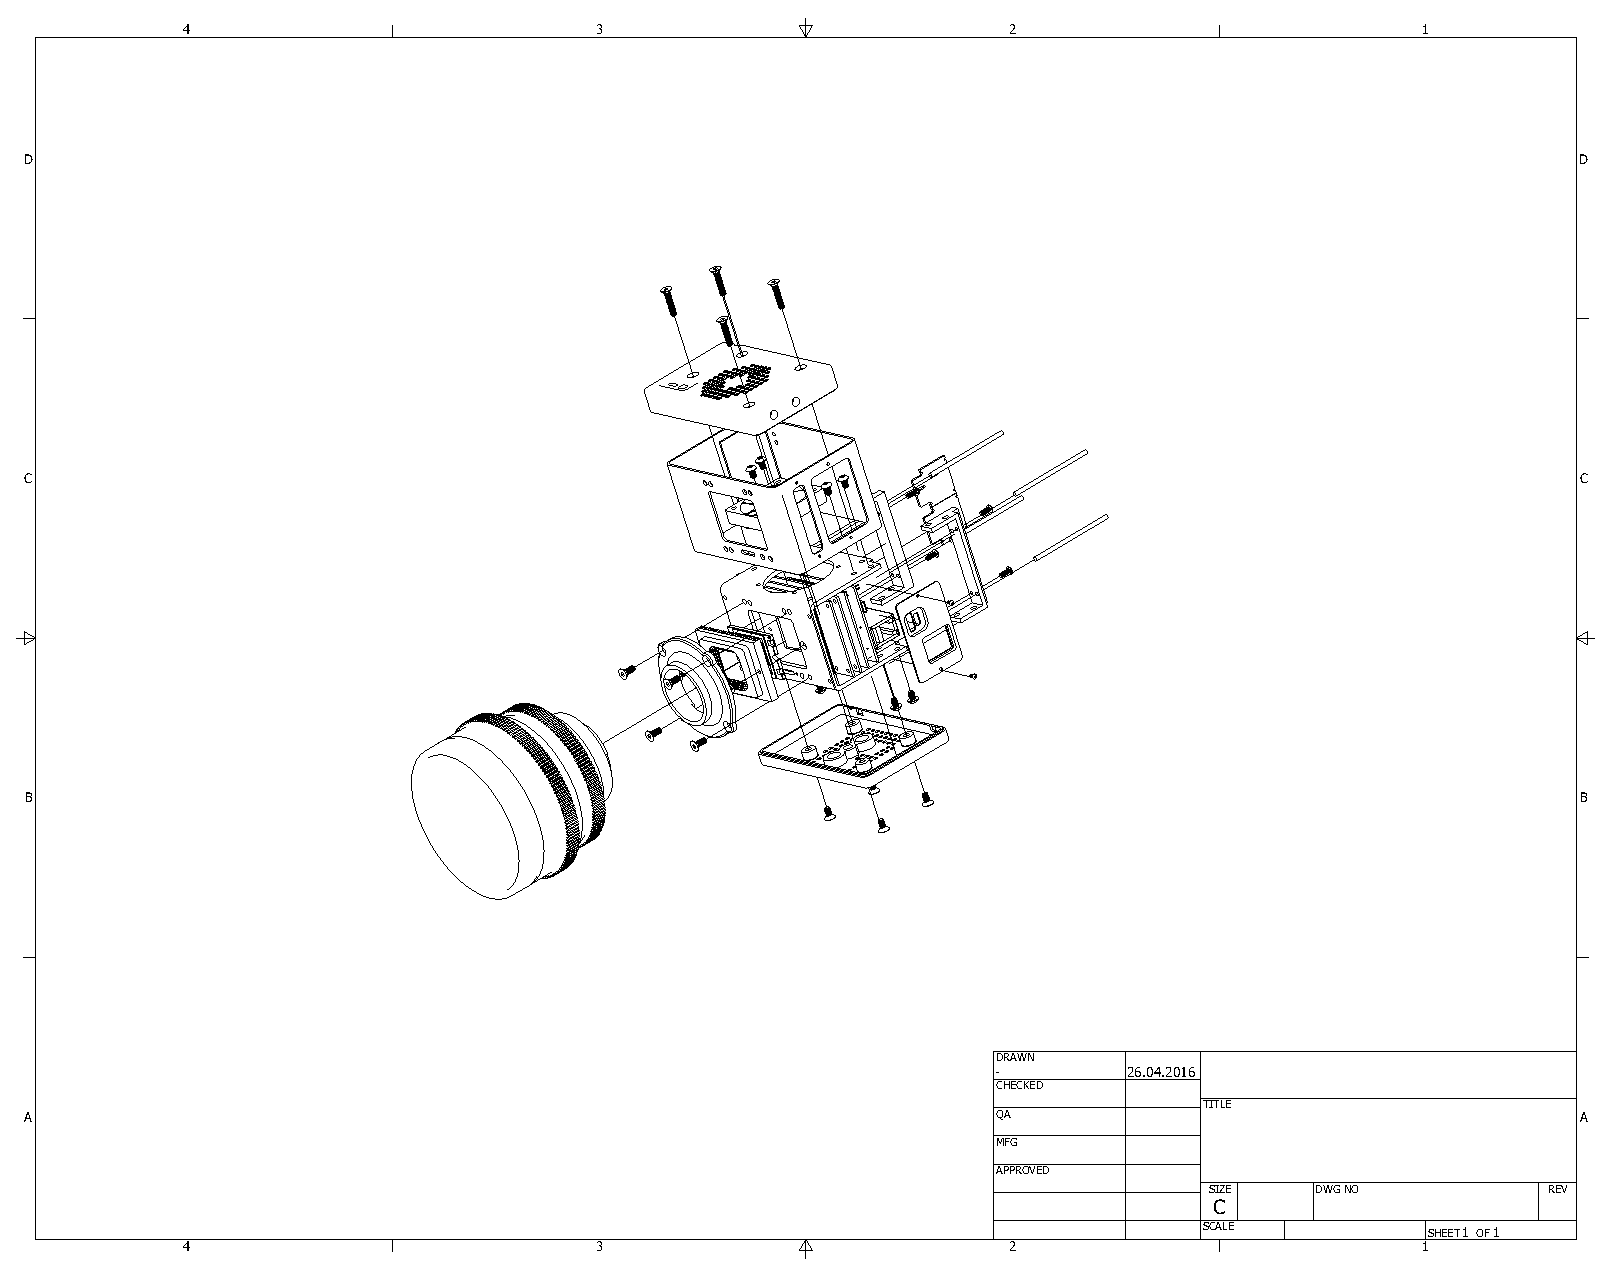
\includegraphics[height=13cm]{images/explosion-full}\\

\textbf{AXIOM Beta User Guide}\\

Permission is granted to copy, distribute and/or modify this document under the terms of the Creative Commons Attribution 4.0 International Public License (CC BY-SA 4.0).\\

Published by apertus° Association.\\


For more information, email team@apertus.org or visit \href{https://apertus.org}{apertus.org}

\end{titlepage}

\tableofcontents

\vspace*{\fill}
\textbf{Note:} In some instances the instructions we have prepared are written in a manor that can be followed by people without a deep technical knowledge. If you are an advanced user please keep this in mind.\\
\\This document has been compiled using LaTeX and its files are stored in the apertus GitHub repository here. If you choose to make any changes to this document please notify a member of the Team so that those changes can be implimented into instances of this guide that are being made available in other locations and formats eg. the project's Wiki page.

\newpage

\section{General Informaion}


\textbf{Notes on Userspace:} Arch Linux comes with systemd, which has one advantage that the boot process is incredibly fast. Standard tools such as sshd and dhcpcd have been preinstalled.\\

One idea to store camera relevant parameters inside the camera and provide access from most programming languages is to use a database like \href{http://en.wikipedia.org/wiki/Berkeley_DB}{http://en.wikipedia.org/wiki/Berkeley\_DB}


\subsection{AXIOM Beta Connector Overview}
	\subsection{Mountpoints}
	\subsection{Accessories and connected devices}
	



\section{Operating Basics}

\subsection{Prepare your AXIOM Beta for use}

Use a micro-USB cable to connect the camera's MicroZed development board (USB UART) to a computer. The MicroZed board is the backmost, red PCB. (There is another micro-USB socket on the Power Board, but that is the JTAG Interface.)\\

1. Connect the ethernet port on the MicroZed to an ethernet port on your computer. You might have to use an ethernet adapter on newer, smaller machines which come without a native ethernet port.\\ 

2. Connect the AC adapter to the camera's Power Board. (The power cord plugs into an adapter that connects to the Power Board; to power the camera off at a later point, you need not disconnect the adapter from the board but can just unplug the cord from the adapter.)


\subsection{Prepare your computer for use with AXIOM Beta}

\textbf{Overview -} To communicate with your AXIOM Beta camera, you will send it instructions via your computer's command line.\\

In case you have not worked with a shell (console, terminal) much or ever before, we have prepared detailed instructions to help you get you set up. The steps which need to 	be taken to prepare your machine sometimes differ between operating systems, so pick the ones that are applicable to you(r system). \\

Note that dollar signs placed in front of commands are not meant to be typed in but denote 	the command line prompt (a signal indicating the computer is ready for user input). It is used in documentation to differentiate between commands and output resulting from commands. The prompt might look different on your machine (e.g. an angled bracket >) and be preceded by your user name, computer name or the name of the directory which you are currently inside.



\subsubsection{USB to UART Drivers}

For the USB connection to work, you will need drivers for bridging USB to UART (USB to serial). (Under Linux this works out of the box in most 	distributions) for other operating systems they can be 

\hyperlink{https://www.silabs.com/products/development-tools/software/usb-to-uart-bridge-vcp-drivers}{downloaded}
downloaded from e.g. Silicon Labs' website – pick the software provided for your OS and install it. \\

\subsubsection{Serial Console}
\paragraph{Linux Setup}
\paragraph{MAC OSX Setup}
\paragraph{Minicom Configuration}
\subsubsection{Serial connection (via USB)}
\paragraph{Connect using Minicom}\mbox{}\\
Note that you will not be able to use the terminal window you initiate the serial connection in for anything else (it needs to remain open while you access the camera), so it might make sense to open a separate window just for this purpose.

With minicom installed and properly configured, all you need to do is run the following command to start it with the correct settings:

\begin{lstlisting}[language=bash,frame=none,xleftmargin=.25in,belowskip=2em, aboveskip=2em]
$ minicom -8 USB0
\end{lstlisting}

On successful connection, you will be prompted to enter user credentials (which are needed to log into the camera).

If your terminal remains blank except for the minicom welcome screen/information about your connection settings, try pressing enter. If this still does not result in the prompt for user credentials – while testing, we discovered the initial connection with minicom does not always work – disconnect the camera from the power adapter, then reconnect it: in your minicom window you should now see the camera's operating system booting up, followed by the login prompt. (From then on, connecting with minicom should work smoothly and at most require you to press enter to make the login prompt appear.)

\paragraph{Connect using Screen}
\paragraph{Disconnect}
\subsubsection{Ethernet connection (using SSH)}
\paragraph{SSH Keys how-to for Linux and Mac}
\subparagraph{Storage location/Find existing keys}
\subparagraph{SSH key creation}
\paragraph{Get or set IP address}
\paragraph{IP address check}
\paragraph{Set IP address}
\paragraph{Establish a connection via key}
\paragraph{Password-based authentication}
\subsubsection{Start the camera}
\subsubsection{WiFi access point setup}


\section{Writing Images}
\subsection{Capture Still Images}
\subsubsection{Parameters}
\subsection{Image Overlays}
\subsubsection{Internals}
\subsubsection{Prepare Images}
\subsubsection{mimg}

\section{Changing Camera Parameters}
\subsection{Settings CMV12000 sensor registers}
\subsection{Setting Exposure Time}
\subsection{Setting gain value}
\subsection{Setting Gamma Values}

\section{Image metadata}
\subsection{cmv hist}

\section{Output}
\subsection{HDMI}
\subsubsection{External HDMI Recording}
\subsubsection{Experimental UHD Raw Recording}
\subsubsection{EDL Parser}
\subsubsection{cmv perf3}
\subsection{SDI}
\subsection{Modes}
\subsection{Generator and HDMI Output}
\subsection{Stopping and Starting HDMI Live-stream}

\section{Processing}
\subsection{Image Acquisition Pipeline}
\subsection{HDMI Image Processing/Output Pipeline}
\subsection{SDI Image Processing/Output Pipeline}
\subsection{Image Processing Nodes}

\section{Converting}
\subsection{RAW12 to PGM}
\subsection{RAW12 to DNG}

\section{Maintenance}
\subsection{Firmware Backup}
\subsection{Firmware Restore}
\subsection{Image Sensor cleaning}

\section{Installations}
\subsection{Installing a webserver}
\subsection{Configuring a webserver}
\subsection{Installing AXIOM Beta Web GUI software}

\section{Colour Science}
\subsection{Black Calibration}
\subsection{Pattern Noise}
\subsection{CMV12000 PLR}
\subsection{CMV12000 Response Curves}

\section{Associated Use-cases}
\subsection{Configuration for Photography}

\section{Hardware}
\subsection{PCB Stack Layout}
\subsubsection{Shields}
\subsubsection{Plugin Modules}
\subsubsection{EEPROM}
\subsection{PCB Revision Links}
\subsection{Power Supply}
\subsubsection{AC Power Supply}
\subsubsection{DC Power Supply}
\subsubsection{Active Battery Mount}
\subsection{Enclosure}
\subsubsection{Skeleton}
\subsubsection{Simple Enclosure}
\subsubsection{Transparent Acrylic Enclosure}
\subsection{Optical Information}
\subsubsection{Lens Mount}
\subsubsection{Lens Mount Overviews}
\subsubsection{Infra Red / Ultra Violet Cut-off Filter}
\subsubsection{Optical Low-pass Filter (OLPF)}

\section{Support}
\subsection{Contact Details and Communication Channels}
\subsection{Regional Communities}
\subsection{Useful Links}



%\\Test


\begin{lstlisting}
    1: lo: <LOOPBACK,UP,LOWER_UP> mtu 65536 qdisc noqueue state UNKNOWN group default 
        link/loopback 00:00:00:00:00:00 brd 00:00:00:00:00:00
        inet 127.0.0.1/8 scope host lo
           valid_lft forever preferred_lft forever
        inet6 ::1/128 scope host 
           valid_lft forever preferred_lft forever
    2: eth0: <BROADCAST,MULTICAST,UP,LOWER_UP> mtu 1500 qdisc pfifo_fast state UP group default qlen 1000
        link/ether 00:0a:35:00:01:26 brd ff:ff:ff:ff:ff:ff
        inet 192.168.0.9/24 brd 192.168.0.255 scope global dynamic eth0
           valid_lft 172739sec preferred_lft 172739sec
        inet6 fe80::20a:35ff:fe00:126/64 scope link 
           valid_lft forever preferred_lft forever
\end{lstlisting}


\begin{lstlisting}
    cd ~/.ssh/
    cp authorized_keys authorized_keys.orig
\end{lstlisting}


ghgffghfg

\end{document}
